\documentclass[11pt]{article}

\usepackage{fontspec}
\usepackage{amsmath}
\usepackage{polyglossia}
\setmainlanguage{turkish}
\usepackage{geometry}
\geometry{a4paper, margin=2.5cm}
\usepackage{graphicx}
\usepackage{booktabs}
\usepackage{float}
\usepackage{caption}
\usepackage{xcolor}
\usepackage{hyperref}
\hypersetup{colorlinks=true, linkcolor=blue, urlcolor=blue}

\graphicspath{{figures/}}

\title{\textbf{YKS Cevap Anahtarı Örüntü Analizi ve\\
Şık Tahmini: Bir ``Sallamasyon'' Çalışması}}
\author{Hamza Yiğit Kültür\\[2pt]
\small \texttt{sallamasyon-yks} --- NVIDIA GH200 (Grace 72-core + H100)}
\date{\today}

\begin{document}
\maketitle

\begin{abstract}
\noindent
Bu çalışma, 2018--2024 yılları arasındaki YKS (TYT ve AYT) sınavlarının
cevap anahtarlarını analiz ederek, ÖSYM'nin doğru cevap dağılımında
sömürülebilir bir istatistiksel örüntü olup olmadığını araştırır. 16 adet
resmî sınav kitapçığı PDF'inden koordinat-tabanlı bir çıkarım yöntemiyle
toplam \textbf{2034} geçerli cevap (İPTAL hariç) elde edilmiştir. Şık
dağılımının düzgüne yakın olduğu (ki-kare $=3.35$, anlamsız), ancak
\emph{ardışık aynı şıkkın belirgin biçimde nadir olduğu} ($\%13.14$, rastgele
beklenen $\%20$) bulunmuştur. 2025 sınavı bağımsız değerlendirme (evaluation)
seti olarak kullanılmış; istatistiksel baseline'lar ile dört sinir ağı
mimarisi (MLP, CNN, GRU, Transformer) karşılaştırılmıştır. En iyi sonucu
\textbf{GRU} ($\%24.88 \pm 3.04$) vermiştir; bu, rastgele tahminin
($\%19.93$) üzerinde fakat mütevazı bir kazanımdır. Sonuçlar, YKS
cevaplarının büyük ölçüde rastgele olduğunu, tek anlamlı sinyalin
``tekrar kaçınması'' olduğunu göstermektedir.
\end{abstract}

\section{Giriş ve Motivasyon}
Çoktan seçmeli sınavlarda, cevabı bilinmeyen sorularda boş bırakmak yerine
istatistiksel olarak en olası şıkkı işaretlemek (halk arasında
\emph{``sallamak''}) yaygın bir stratejidir. Bu çalışmanın amacı, geçmiş YKS
cevap anahtarlarından öğrenilebilecek bir örüntü olup olmadığını
\emph{dürüst ve tekrarlanabilir} biçimde test etmektir. Beklentimiz
baştan düşüktü: iyi tasarlanmış bir sınavın cevap anahtarı, tahmin
edilemez (rastgeleye yakın) olmalıdır. Bu rapor, bu beklentinin büyük
ölçüde doğrulandığını ancak küçük bir istisnanın bulunduğunu belgeler.

\section{Veri ve Çıkarım Yöntemi}
Veri seti, ÖSYM'nin resmî sınav kitapçıklarından oluşur (2018--2024 eğitim,
2025 değerlendirme). Cevap anahtarları her PDF'in son sayfasında, çok
sütunlu bir düzende ve üzerinde çapraz filigran (watermark) metni bulunan
biçimde yer alır. Bu filigran, naif metin çıkarımını bozmaktadır.

\paragraph{Koordinat-tabanlı çıkarım.}
\texttt{pdftotext -bbox-layout} ile her kelimenin piksel koordinatları
alınmış; tek harfli A--E hücrelerinin $x$ koordinatları kümelenerek ders
sütunları filigrandan bağımsız biçimde tespit edilmiştir. Her soru numarası,
$y$ koordinatına göre ilgili cevapla eşleştirilmiştir. Bu yöntem, naif
yaklaşımın başarısız olduğu AYT 2022 (sütun dağılması) ve filigran
çakışması (TYT 2020, 18.\ soru) durumlarını çözmüştür. İptal edilen sorular
(TYT 2019'da 1 adet) ayrıca işaretlenmiştir. Tüm 16 PDF, otomatik doğrulama
katmanından (her ders için 1--$N$ kesintisiz soru kontrolü) \textbf{sıfır
uyarı} ile geçmiştir.

\section{Keşifsel Analiz}

\subsection{Şık Dağılımı}
Genel şık dağılımı düzgüne oldukça yakındır (Tablo~\ref{tab:dist},
Şekil~\ref{fig:genel}). Düzgün dağılıma karşı yapılan ki-kare testi
$\chi^2 = 3.35$ değerini vermiştir; bu, $df=4$ için $\%5$ kritik değeri olan
$9.49$'un altındadır. Dolayısıyla \emph{``belirli bir şık daha sık çıkar''
hipotezi istatistiksel olarak reddedilir}. Pratik sonuç: her soruya kör
biçimde tek bir şık (ör.\ ``hep D'') işaretlemek, rastgeleye karşı anlamlı
bir avantaj sağlamaz.

\begin{table}[H]
\centering
\caption{Genel şık dağılımı (\%), 2018--2024, $n=2034$.}
\label{tab:dist}
\begin{tabular}{lccccc}
\toprule
& A & B & C & D & E \\
\midrule
Genel & 19.27 & 20.40 & 20.50 & 20.99 & 18.83

\\
\bottomrule
\end{tabular}
\end{table}

\begin{figure}[H]
\centering
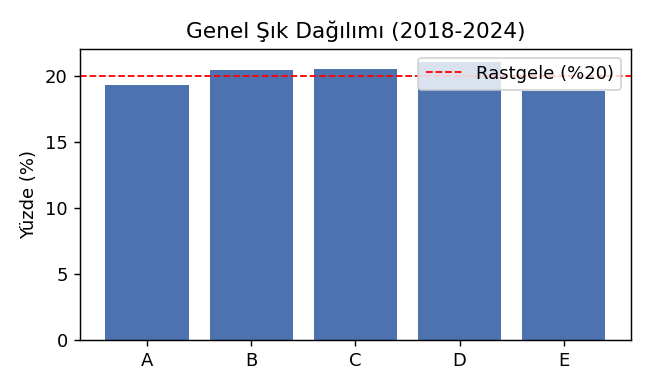
\includegraphics[width=0.62\textwidth]{dagilim_genel.png}
\caption{Genel şık dağılımı. Kırmızı kesikli çizgi rastgele beklentiyi
($\%20$) gösterir. Tüm şıklar bu çizgiye yakındır.}
\label{fig:genel}
\end{figure}

\begin{table}[H]
\centering
\caption{Ders bazlı şık dağılımı (\%).}
\label{tab:subdist}
\begin{tabular}{lccccc}
\toprule
Ders & A & B & C & D & E \\
\midrule
Edebiyat-Sosyal1 & 22.1 & 16.4 & 23.2 & 18.9 & 19.3 \\
Fen & 18.6 & 20.0 & 19.8 & 21.9 & 19.8 \\
Matematik & 18.8 & 21.6 & 20.9 & 20.8 & 17.9 \\
Sosyal & 17.2 & 21.3 & 20.7 & 20.1 & 20.7 \\
Sosyal2 & 19.6 & 21.4 & 19.6 & 21.7 & 17.7 \\
Türkçe & 19.4 & 20.8 & 19.0 & 21.9 & 19.0

\\
\bottomrule
\end{tabular}
\end{table}

\subsection{Ardışık Tekrar: Tek Gerçek Sinyal}
En çarpıcı bulgu, ardışık (peş peşe) soruların aynı şıkka sahip olma
oranıdır: \textbf{yalnızca $\%13.14$}, rastgele beklenen $\%20$'nin belirgin
biçimde altında. Veri setinde gözlemlenen \emph{maksimum ardışık tekrar 3}'tür;
yani aynı şık asla 4 kez üst üste gelmemiştir. Bu, ÖSYM'nin cevap anahtarını
oluştururken bilinçli ya da örtük olarak ``tekrar kaçınması'' uyguladığını
düşündürür. Markov geçiş matrisinde (Şekil~\ref{fig:markov}) bu durum,
köşegen değerlerinin (aynı şıkka geçiş) düşük olmasıyla açıkça görülür.
\textbf{Bu örüntü, bu çalışmadaki tek sömürülebilir sinyaldir.}

\begin{figure}[H]
\centering
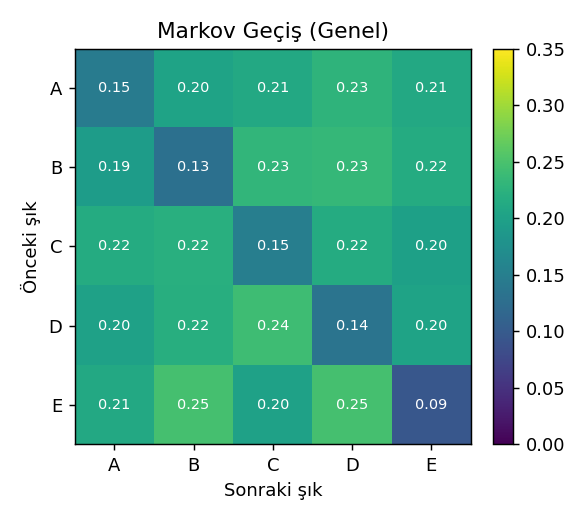
\includegraphics[width=0.5\textwidth]{markov_genel.png}
\caption{Markov geçiş matrisi $P(\text{sonraki}\mid\text{önceki})$. Köşegen
(aynı şıkka geçiş) tutarlı biçimde $0.20$'nin altındadır; ortalama $0.131$.}
\label{fig:markov}
\end{figure}

\section{Veri Seti ve Eğitim Kurgusu}
\paragraph{Veri.} Ham veri, ÖSYM'nin 16 resmî sınav kitapçığı PDF'idir
(TYT ve AYT, 2018--2025). Cevap anahtarları, koordinat-tabanlı bir çıkarıcı
ile elde edilmiş ve $\{$yıl, sınav, ders, soru\_no, şık$\}$ şemasında
yapılandırılmıştır. Eğitim seti yalnızca \textbf{2018--2024}'tür: İPTAL edilen
sorular çıkarıldıktan sonra \textbf{2034} cevap, $56$ adet (yıl, sınav, ders)
dizisinden oluşur. \textbf{2025} sınavı ($291$ cevap) eğitime hiç katılmayan
bağımsız değerlendirme setidir.

\paragraph{Girdi temsili.} Her cevap, $A$--$E$ için $\{0,1,2,3,4\}$ tamsayı
etiketine eşlenir. Bir ``dizi'', tek bir (yıl, sınav, ders) testinin soru
sırasına göre dizilmiş şık etiketleridir (ör. TYT Matematik için 40 elemanlı).
Ders adı bir kategorik öznitelik olarak gömme (embedding) ile temsil edilir.

\paragraph{Tahmin senaryosu.} Bir dizide her pozisyondaki şık, geçmiş (bilinen)
şıklardan tahmin edilir---``önceki cevaplar belli, sonrakini salla'' senaryosu.
Dizisel modeller \emph{nedensel} (causal) çalışır: pozisyon $i$ yalnızca
$<i$ konumları görür, böylece geleceğe sızıntı olmaz.

\section{Model Mimarileri}
Tüm modeller PyTorch ile yazılmış ve NVIDIA GH200 üzerinde eğitilmiştir.
Sinir ağlarının ortak hiperparametreleri: gömme/gizli boyut $d_{\text{model}}=64$
(MLP'de gizli katman $128$), optimizasyon AdamW (öğrenme oranı $2\times10^{-3}$,
ağırlık çürümesi $10^{-3}$), kayıp çapraz-entropi, dropout $0.3$. Her model
$10$ farklı tohum (seed) ile eğitilip ortalama $\pm$ standart sapma
raporlanır.

\paragraph{Baseline'lar (sinir ağı değil).} (i) \emph{Rastgele}: düzgün
$5$-sınıf tahmin. (ii) \emph{En Sık Şık}: ders bazlı en sık şıkkı her soruya
verir. (iii) \emph{Pozisyonel}: $P(\text{şık}\mid\text{ders}, \text{soru\_no})$
argmax. (iv) \emph{Markov}: $P(\text{sonraki}\mid\text{önceki})$ geçiş
matrisi (Laplace düzeltmeli) ile argmax.

\paragraph{MLP.} Tablo-tabanlı ileri-beslemeli ağ. Girdi: ders gömmesi
($8$ boyut) $+$ normalize soru numarası $+$ son üç şıkkın gömmeleri
($3\times 8$). İki gizli katman ($128$, ReLU, dropout) ardından $5$-sınıf
softmax. Diziyi bütün olarak görmez; yalnızca yerel öznitelikleri kullanır.

\paragraph{CNN (nedensel).} Şık dizisini token gömmeleri $+$ konum gömmeleri
$+$ ders gömmesi ile temsil eder. İki adet $1$-boyutlu evrişim katmanı
(çekirdek $3$, $d_{\text{model}}=64$) uygular; \emph{sol-pad} ile geleceğe
bakması engellenir (nedensellik). Her pozisyon için $5$-sınıf çıktı üretir.

\paragraph{GRU (nedensel).} Aynı gömme girdisi üzerinde $2$ katmanlı GRU
(gizli boyut $64$, dropout $0.3$). RNN doğası gereği yalnızca geçmişe baktığı
için nedensellik kendiliğinden sağlanır. Her zaman adımında $5$-sınıf çıktı.

\paragraph{Transformer (nedensel).} $2$ kodlayıcı katmanı, $4$ dikkat başlığı,
ileri-besleme boyutu $4\,d_{\text{model}}$, GELU aktivasyonu. \emph{Üçgensel
nedensel maske} ile pozisyon $i$ yalnızca $\le i$ konumlara dikkat eder.
Token, konum ve ders gömmeleri toplanarak girdi oluşturulur.

\section{Değerlendirme Protokolü}
\textbf{Doğruluk tanımı.} Bir modelin doğruluğu, 2025 test setinde doğru
tahmin edilen soru sayısının toplam soru sayısına oranıdır
($\text{doğruluk}=\tfrac{\text{doğru tahmin}}{\text{toplam soru}}$), yüzde
olarak verilir. Rastgele beklenti $5$ şık için $\%20$'dir.

\textbf{Tur sayısı.} Sinir ağları (MLP, CNN, GRU, Transformer) rastgele
başlatmaya duyarlı olduğundan, her biri \textbf{$10$ bağımsız tohum (seed)}
ile eğitilip değerlendirilir; tabloda \emph{ortalama $\pm$ standart sapma}
($10$ tur üzerinden) raporlanır. Baseline'lar deterministiktir (Rastgele
hariç), tek değer verir. Hiçbir sonuç tek-atış değildir.

\section{Sonuçlar}
Dört baseline ile dört sinir ağı 2025'te karşılaştırılmıştır.

\begin{table}[H]
\centering
\caption{2025 değerlendirme doğrulukları. ``Eğitim'' sütunu eğitim setindeki
doğruluğu gösterir; sinir ağlarındaki yüksek eğitim doğruluğu aşırı öğrenmeye
(overfitting) işaret eder.}
\label{tab:results}
\begin{tabular}{llcc}
\toprule
Model & Tür & 2025 Doğruluk (\%) & Eğitim (\%) \\
\midrule
Rastgele & Baseline & 19.93 & -- \\
EnSıkŞık & Baseline & 21.99 & -- \\
Pozisyonel & Baseline & 18.56 & -- \\
Markov & Baseline & 21.65 & -- \\
MLP & Sinir Ağı & 18.25$\pm$1.57 & 45.0 \\
CNN & Sinir Ağı & 20.03$\pm$2.15 & 96.5 \\
\textbf{GRU} & Sinir Ağı & \textbf{24.88$\pm$3.04} & 96.1 \\
Transformer & Sinir Ağı & 22.41$\pm$2.18 & 96.6

\\
\bottomrule
\end{tabular}
\end{table}

\begin{figure}[H]
\centering
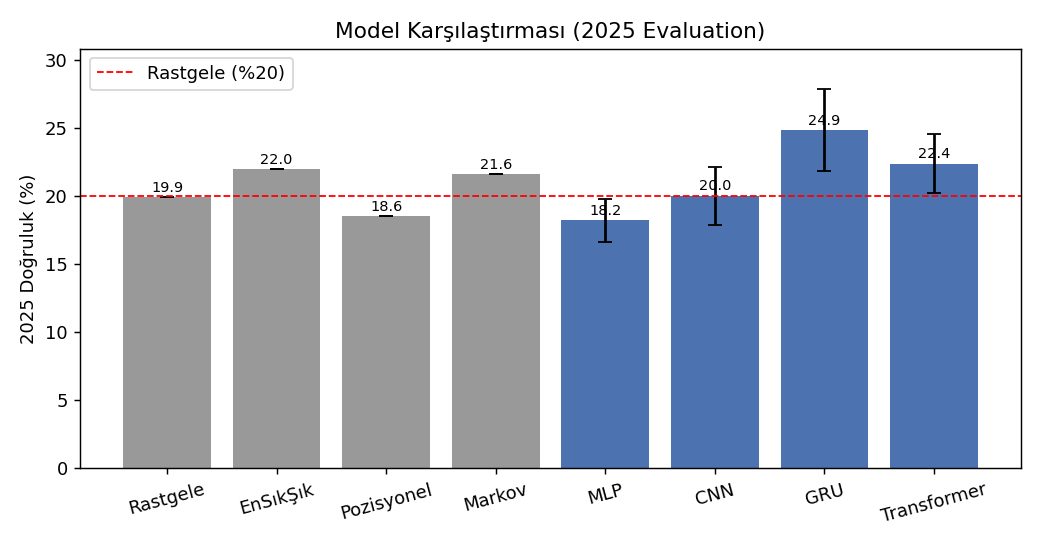
\includegraphics[width=0.85\textwidth]{sonuc_karsilastirma.png}
\caption{Model karşılaştırması (2025). Gri: baseline, mavi: sinir ağı.
Hata çubukları 10 tohumun standart sapmasıdır. Kırmızı çizgi rastgele
($\%20$) seviyesini gösterir.}
\label{fig:sonuc}
\end{figure}

\section{Tartışma}
Sonuçlar (Tablo~\ref{tab:results}, Şekil~\ref{fig:sonuc}) birkaç net mesaj
verir:
\begin{itemize}
  \item \textbf{Aşırı öğrenme baskındır.} MLP, CNN, GRU ve Transformer
  eğitim setinde $\%45$--$\%97$ doğruluğa ulaşırken değerlendirmede
  $\%18$--$\%25$ bandında kalır. Veri küçük (2034 örnek) ve gerçek sinyal
  zayıf olduğundan, yüksek kapasiteli modeller eğitim verisini ezberler.
  \item \textbf{Pozisyonel bilgi işe yaramaz.} Pozisyonel baseline
  ($\%18.56$) rastgelenin dahi altındadır; ``$k$.\ soru genelde X şıkkıdır''
  diye bir kural yoktur.
  \item \textbf{Tek kazanç tekrar kaçınmasından gelir.} Markov ($\%21.65$)
  ve onun zengin versiyonu olan GRU ($\%24.88 \pm 3.04$) baseline'ı geçer.
  GRU'nun avantajı, ardışık tekrar kaçınması örüntüsünü Markov'dan daha
  esnek modellemesinden kaynaklanır.
  \item \textbf{Kazanım mütevazı ve gürültülüdür.} En iyi model bile
  rastgelenin yalnızca $\sim 5$ puan üzerindedir ve standart sapması yüksektir
  ($\pm 3$). Bu, pratikte ``her boş soruda $\sim$\%5 ekstra isabet'' demektir;
  garanti değil, beklenen değer.
\end{itemize}

\paragraph{Donanım notu.} Modeller NVIDIA GH200 üzerinde eğitildi. Dürüst
olmak gerekirse, problemin ölçeği bu donanımın kapasitesinin çok altındadır;
tüm model zoo saniyeler içinde eğitilmiştir. GH200 burada bir gereklilik
değil, erişilebilir bir araç olarak kullanılmıştır.

\section{Sonuç}
YKS cevap anahtarları, tasarım amacına uygun biçimde \emph{büyük ölçüde
tahmin edilemezdir}. Şık dağılımı düzgüne yakındır ve konuma bağlı bir
örüntü yoktur. Tespit edilebilen tek yapısal özellik, aynı şıkkın peş peşe
nadiren tekrarlanmasıdır; bu da en fazla birkaç puanlık bir avantaj sağlar.
``Sallamasyon'' için pratik öneri sadedir: \emph{bilinen komşu cevaplardan
farklı bir şık seçmek}, kör rastgeleye göre küçük ama tutarlı bir kazanç
getirir---gerisi şanstır.

\paragraph{Tekrarlanabilirlik.} Tüm kod ve veri açık biçimde
\texttt{scripts/} ve \texttt{data/processed/} altındadır. İşlem hattı:
\texttt{extract\_answers.py} $\rightarrow$ \texttt{analyze.py}
$\rightarrow$ \texttt{train.py} $\rightarrow$ \texttt{build\_report.py}.

\end{document}
